% Voir recommandations ED SVS !!!!!! puis adapter

\pagestyle{empty}

% Les logos en tête


\includegraphics[scale=1, height=1.7cm]{0_Liminaires/Images/UBX_logo.png}
\hfill

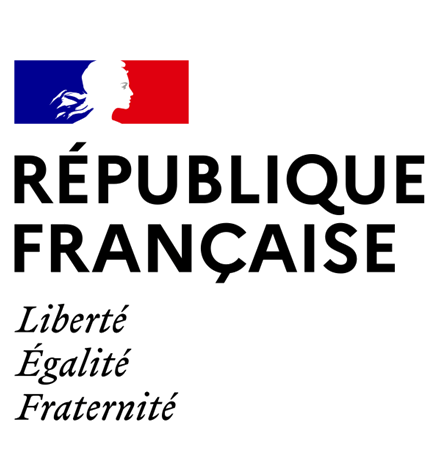
\includegraphics[scale=1, height=1.7cm]{0_Liminaires/Images/RF.png} %  remplacer par logo UMR (+ ISVV ?)
\hfill

\begin{center}
\doublespacing
\begin{Large}

THÈSE PRÉSENTÉE\\ POUR OBTENIR LE GRADE DE \\
{\LARGE \textbf{DOCTEUR\\DE L'UNIVERSITÉ DE BORDEAUX} } \\
\vspace{0.55cm}
ECOLE DOCTORALE SCIENCES DE LA VIE ET DE LA SANTÉ\\
{\normalsize Spécialité OENOLOGIE} \\
\vspace{0.55cm}
Par \textbf{Guillaume Séraphin BLANC LELEU} \\
\vspace{0.55cm}
{\Large Titre.}
\end{Large}
\vspace{0.55cm}
\begin{normalsize}
\begin{singlespace}
Sous la direction de : \textbf{Tristan RICHARD}\\
Responsable scientifique : \textbf{...}
\end{singlespace}
\end{normalsize}
\end{center}
\vfill
\begin{center}
{\large Soutenue le x novembre 2025 }\\    
\end{center}
\vfill
Membres du jury :
\begin{table}[b]
\centering
\makebox[\textwidth]{%
\begin{tabular}{lllr}
Mme Prénom NOM & Grade & Université & Rapporteuse \\
Mme Prénom NOM & Grade & Université & Fonction \\
Mme Prénom NOM & Grade & Université & Fonction \\
Mme Prénom NOM & Grade & Université & Fonction \\
Mme Prénom NOM & Grade & Université & Fonction \\
\end{tabular}
}
\end{table}

\thispagestyle{empty}
\vspace*{0pt}
\vfill

\afterpage{\blankpage}
\newpage

\begin{small}
\begin{singlespace}
\begin{center}
\textbf{Titre.}
\end{center}
\textbf{Résumé :} 
...

L.\newline
\\
\textbf{Mots-clés :} ... \\

%\noindent\rule{\textwidth}{1pt}
\noindent\makebox[\linewidth]{\rule{\textwidth}{0.4pt}}

\vfill
% \selectlanguage{french}
\begin{center}
    \textbf{Unité de recherche}\\
UMR 1366 OENO, 33140 Villenave-d'Ornon, France.
\end{center}

\afterpage{\blankpage}
\newpage
% \selectlanguage{english}

\begin{center}
\textbf{Title english.}
\end{center}
\textbf{Abstract:} 
...
\\
\newline
\textbf{Keywords:} ... \\

\noindent\makebox[\linewidth]{\rule{\textwidth}{0.4pt}}

\vfill
% \selectlanguage{french}
\begin{center}
    \textbf{Reasearch unit}\\
UMR 1366 OENO, 33140 Villenave-d'Ornon, France.
\end{center}
\end{singlespace}
\end{small}